\documentclass[a4paper]{article}

\usepackage[utf8]{inputenc}
\usepackage[T1]{fontenc}
\usepackage{textcomp}
\usepackage{listings}
\usepackage{lmodern}
\usepackage{amsfonts}
\usepackage{titling}
\usepackage{lipsum}
\usepackage[left=1in, right=1in, bottom=1in, top=1in]{geometry}
\usepackage{mathtools}
\usepackage{amsthm}
\usepackage{tcolorbox}
\usepackage{hyperref}
\usepackage{xcolor}
\usepackage{graphicx}
\usepackage{makeidx}
\usepackage{tikz}
\usepackage{cases}
\usepackage{apacite}
\usepackage{tkz-berge}
\usepackage{lastpage}
\usepackage{fancyhdr}
\pagestyle{fancy} 
\usepackage{url}
\usepackage{tgtermes}
\usepackage{algorithm2e}
\usepackage{sectsty}
\usepackage{subcaption}
\usepackage{setspace}
\usepackage{float}
\usepackage{amsmath, amssymb}
\rhead{Page~\thepage~of~\pageref{LastPage}.}
\cfoot{}

% figure support
\usepackage{import}
\usepackage{xifthen}
\pdfminorversion=7
\usepackage{pdfpages}
\usepackage{transparent}
\newcommand{\incfig}[2][1]{%
    \def\svgwidth{#1\columnwidth}
    \import{./figures/}{#2.pdf_tex}
}

%mathstyling
\theoremstyle{plain}
\newtheorem{thm}{Theorem}[section]
\newtheorem{lem}[thm]{Lemma}
\newtheorem{prop}[thm]{Proposition}
\newtheorem*{cor}{Corollary}

\theoremstyle{definition}
\newtheorem{defn}{Definition}[section]
\newtheorem{conj}{Conjecture}[section]
\newtheorem{exmp}{Example}[section]
\newtheorem{axiom}{Axiom}
\theoremstyle{remark}
\newtheorem*{rem}{Remark}
\newtheorem*{note}{Note}

\pdfsuppresswarningpagegroup=1

\begin{document}
	\begin{titlepage}
	\begin{center}
	\large
	University of Warwick \\
	Department of Computer Science \\
	\huge
	\vspace{50mm}
	\rule{\linewidth}{0.5pt} \\
	CS132: Computer Organisaton \& Architecture \\
	\vspace{5mm}
	\Large
	Coursework 2
	\rule{\linewidth}{0.5pt}
	\vspace{5mm}
	\begin{figure}[H]
	\centering
	
\includegraphics[width=0.4\textwidth]{crest_black.eps}
	\end{figure}
	\vspace{33mm}
	2108182\\
	Cem Yilmaz\\
	\today
	\end{center}
	\end{titlepage}
\tableofcontents
\newpage
\section{Introduction}
\subsection{Problem 1}

\subsection{Problem 2}
\section{Problem 1}
\subsection{Power set}
The first problem of coursework $2$ introduces the implementation of a "Power set" in code. However, in order for this code to be written, it is first important to break down as to what requires to actually be defined.
\begin{tcolorbox}[colback=black!3!white,colframe=black!60!white,title=\begin{defn}Power Set \label{Power Set}\end{defn}]
The power set of a finite set $S$, denoted as $2^{S}$, is the set that contains all subsets of $S$ as its elements. Formally, 
\begin{align*}
	2^{S} = \{ X : X \subseteq S \}
\end{align*}
The cardinality of the set (number of elements denoted as $|S|$), is then, as a corollary:
\begin{align*}
	|2^{S}|&=2^{|S|} \\
	       &=\sum_{i=0}^{|S|} {}^{|S|}C_k
\end{align*}
Note that for the sake of this paper, we will not be discussing if $S$ is infinite, as the code will be implemented with the assumption that the input is also finite.
\end{tcolorbox}
\begin{flushleft}
And the intuition behind this corollary is important for our implementation, as it in fact gives us a big hint as to how Problem $1$ could be implemented as code. Consider the sets $S = \{x,y\}$, $S' = \{ x,y,z \}$, $2^{S}$ and $2^{S'}$. In terms of decision trees for their power sets, it would be visualised as the following:
\end{flushleft}
\begin{figure}[H]
    \centering
    \incfig[0.8]{2s}
    \caption{Visualisation of the power set $2^{S}$}
    \label{fig:2s}
\end{figure}
\begin{figure}[H]
    \centering
    \incfig[0.9]{2sprime}
    \caption{Visualisation of the power set $2^{S'}$}
    \label{fig:2sprime}
\end{figure}
\begin{flushleft}
These figures make it apparent as to how the cardinality $|2^{S}| = 2^{|S|}$ precisely works. That is, for each new element to the set $S$, we must add a new branch of yes or no decisions for all previously existing power set elements. When the answer is no to the new element for all branches, we get $2^{S}$. With all answers yes, we obtain $x \in 2^{S} : x \cup z$. \\

Formally, let us define $S' = S \cup \{ \zeta \}$ where $\zeta$ is the new arbitrary element of a finite set $S$. Then, we can obtain the following formula for their power set:
\end{flushleft}
\begin{align*}
	2^{S^{*}} &= \{ x \in 2^S : x \cup \{ \zeta \}\}\\
	2^{S'} &= 2^S \cup 2^{S^{*}}
\end{align*}
\subsection{Pseudocode}
Now that the intuition and the mathematical formula has been well defined, we could write the pseudo code that we will implement into C. This will help us plan the structure of what is to come when writing our code.\\

\begin{algorithm}[H]
	\caption{Power set pseudocode}
	\KwData{User input of elements into our set $S$ }
	\KwResult{A printed $2^{S}$ }

	Begin \\
	Take input from user\;
	Initialise output variable array\;
	\While{Our counter is not at the size of $|S| + 1$ elements}{
		Initialise counter $ = 1$\;
		\eIf{first element}{Add first singleton set to output variable\;}{Add new element to each existing set in output variable and store them in output variable\;}
		counter $=$ counter$+1$\;
	}
	Add empty set to output variable\;
	Print output variable\;
	End
\end{algorithm}

\begin{flushleft}
Now that the pseudocode has been defined, we could move onto the written code and explaining each line's design.
\end{flushleft}
\subsection{Explanation of code design}
This section will require that the file $powerset.c$ is opened as the lines of code that are expressed in this section correspond to the lines of code of that file.
\begin{itemize}
	\item (Lines $8-16$) The definition of a two power was defined to keep the numbers in unsigned integers. This helps reduce code as type casting is not required as the original package assumes the output not to be an integer
	\item (Lines $36-40$) arraySize is converted into integer during the actual method to ensure that the user does not go over and including the number $20$. 
	\item (Lines $52-55$) The sizes of the variables are as following:
		\begin{itemize}
			\item S as input arraySize as this is the amount of elements it holds.
			\item powerSetS as $2^{arraySize}$ as this is the theoretical amount of elements.
			\item powerSetSStar as $\text{arraySize}-1$ because it will only require at maximum have the same amount of elements that exist in $S$ at that time. However, we subtract another $-1$ because we add the empty set separate for our algorithm.
			\item Memory size as $100$ as this is a good amount to assume that the string will not be longer than $99$ characters.
		\end{itemize}
	\item (Lines $104-107$) It was decided that all subsets will be listed in new lines because otherwise it would be a very long singular line and even difficult to read.
\end{itemize}
Assumptions include that the set is finite and is not larger or including cardinality size $20$. The reason for this is because the stack in the CPU is limited to $8mb$. Increasing this value would not necessarily help much, given that the size set grows exponentially. Re-assigning non-default amount to stack by increasing it is also not necessarily better, as it can lead to stack overflow. Furthermore, unsigned int was used as the general type for numbers as we cannot have negative numbers and int is sufficient for the size of arrays that we are working with. Error catching was implemented for cardinality size to ensure a smooth run. The number error catching was re-used from coursework $1$. Pointers for strings were used as it is one of the best and compact methods available in C \cite{pointer} \cite{pointer2}.
\newpage
\subsection{Flowchart}
\begin{figure}[H]
	\centering
	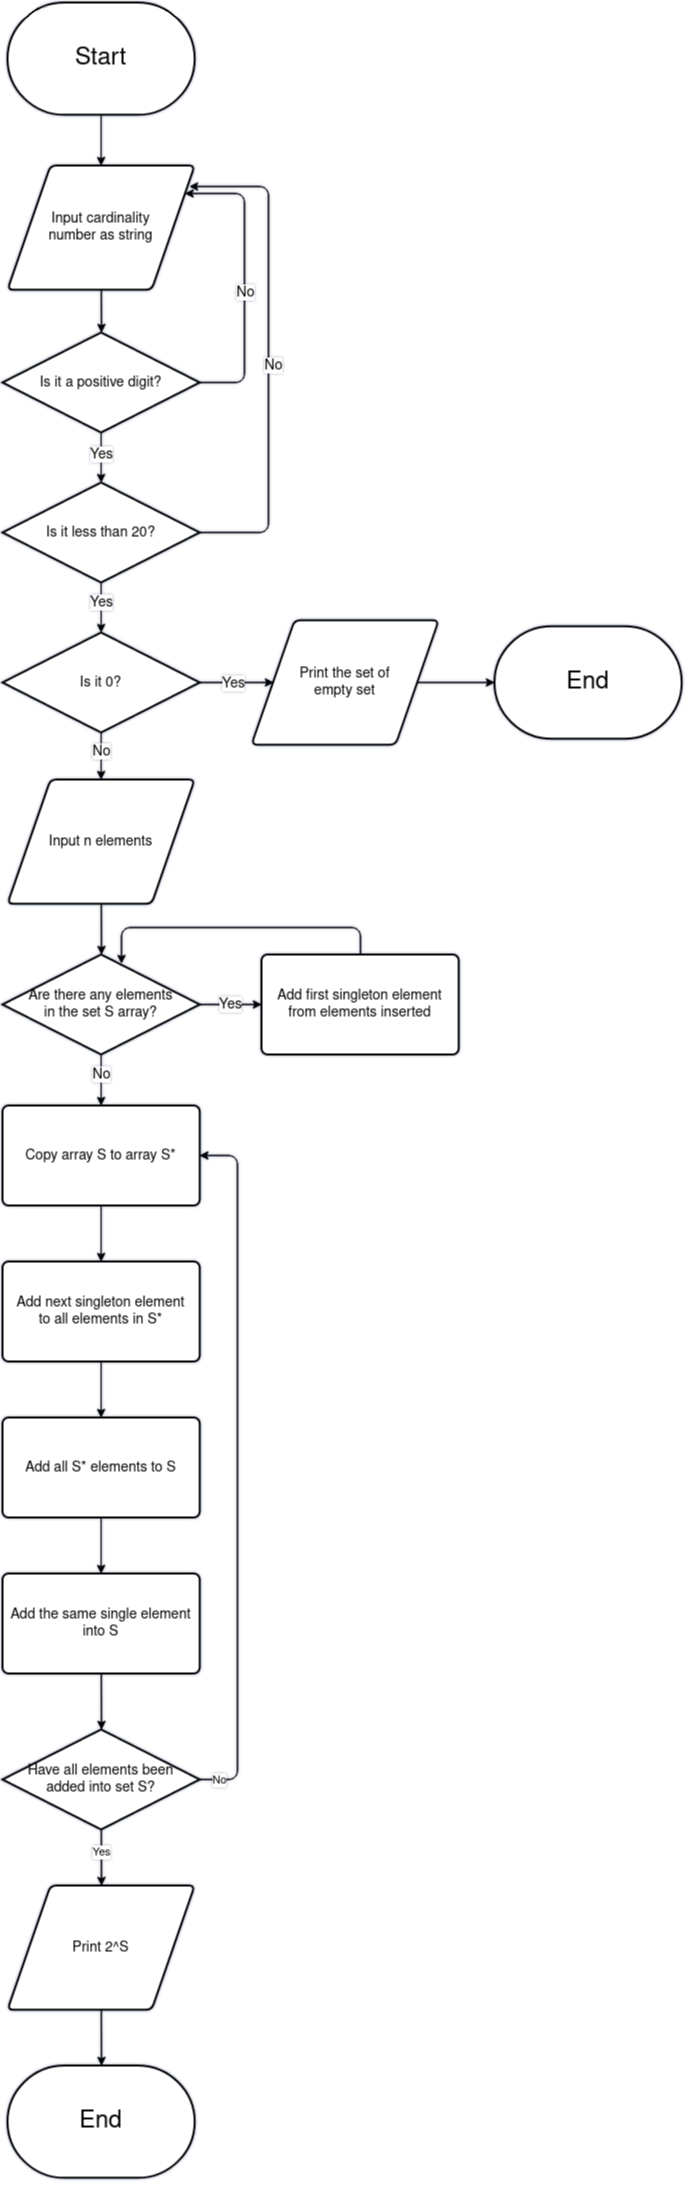
\includegraphics[width=0.45\textwidth]{figures/cs.png}
	\caption{Flowchart of the implemented algorithm}
	\label{fig:algorithm}
\end{figure}
\newpage
\section{Problem 2}
\subsection{Pseudocode}
\subsection{Explanation of code design}
\begin{itemize}
	\item (Lines $20-22$ ) A capacity of $256$ and $128$ was chosen for directory and file respectively as these are likely to be more than enough characters that the user would need.
	\item (Lines $31-35$) It was chose to add the symbol $\backslash$ between the name and the directory input as in a lot of operating systems, including Windows and Linux, when finding directory location with mouse it does not reveal the final slash.
	\item (Lines $60-70$ ) Because a lot of operations/functions require the correct input of of information about the file, a method was added to ensure this by repeatedly asking the user again until it is correct.
	\item (Lines $39-56$ ) This code repeats a lot throughout the file, therefore adding it as a method is sensible. It is used in name input, directory input and forceFixLocation method to ensure give information about whether the user input is a valid input by checking existence.
	\item (Lines $87-107$) Because of the possibly confusing interface due to the presence of high amount of operations/functions that the user can do, a help function was added.
	\item (Lines $203-205$ ) The interface includes an "edit" mode for ease of use of the user. That is, the edit mode would display help for the editing of the file they have selected.
	
\end{itemize}
\subsection{Flowchart}


\newpage
\bibliographystyle{apacite}
\bibliography{bibliography}
	
\end{document}
